\documentclass[a4paper, 16pt]{article}
\usepackage[UTF8]{ctex}
\usepackage{geometry}
\usepackage{graphicx}
\usepackage{setspace}
\usepackage{float}
\usepackage{listings}
\usepackage{xcolor}
\usepackage{multirow}
\lstset{
    numbers=left, 
    numberstyle= \tiny, 
    keywordstyle= \color{ blue!70},
    commentstyle= \color{red!50!green!50!blue!50}, 
    frame=shadowbox, % 阴影效果
    rulesepcolor= \color{ red!20!green!20!blue!20} ,
    escapeinside=``, % 英文分号中可写入中文
    xleftmargin=5em,xrightmargin=5em, aboveskip=2em,
    framexleftmargin=2em
} 
\geometry{left = 1.0 cm, right = 1.0cm, top = 2.0cm, bottom = 2.0cm	}
\title{编译原理第八章(三)}

\author{李鹏辉}

\begin{document}
\maketitle
1.(8.6.1)为下面的每个c语言赋值生成三地址代码
\lstset{language=C}
\begin{lstlisting}
x = a + b * c
a[i] = b[c[i]]
*p++ == *q++
\end{lstlisting}

1)
\begin{table}[H]
\centering
\begin{tabular}{l}
t1 = b * c\\
x = a + t1\\
\end{tabular}
\end{table}

2)
\begin{table}[H]
\centering
\begin{tabular}{l}
t1 = i * 4\\
t2 = c[t1]\\
t3 = t2* 4\\
a[t1] = b[t3]\\
\end{tabular}
\end{table}
3)
\begin{table}[H]
\centering
\begin{tabular}{l}
p = p + 4\\
q = q + 4\\
$*q = *p$\\
\end{tabular}
\end{table}

1.(8.8.1)为图8-17的程序构造寄存器冲突图(干涉图)

根据课本8-18的全局寄存器指派序列图可知\\
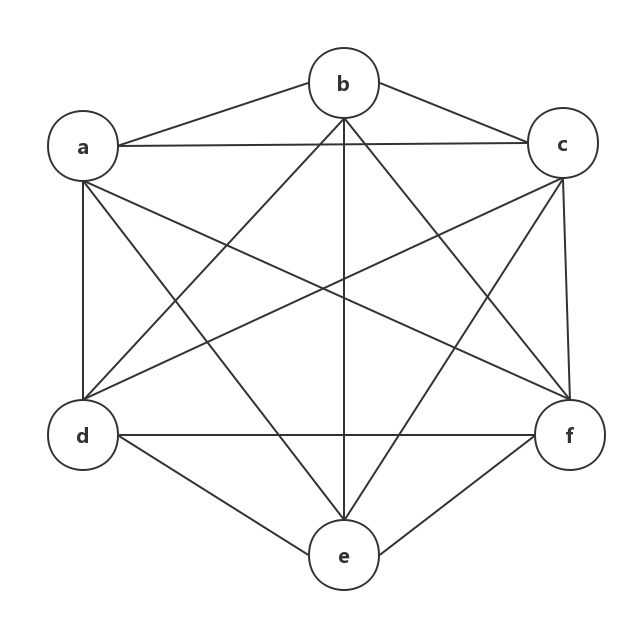
\includegraphics[scale=0.3]{chapter8_hw3_1}
\end{document}